\section{Design and Implementation}
\label{sect:apner_architecture}
As previously mentioned, our main goal in designing polyNER is to slash labeling costs by reducing the time and effort spent by experts to generate training data. 
Rather than labeling entire documents and phrases, annotators label proposed candidate entities to be classified.
%\logan{What is downstream in this metaphor? I also don't think it is a needed detail}\roselyne{ok, removed, it stemmed from the idea in my head about mentioning that our labels can be used by Hong, and others later, picked up from snuba, but probably can be emphasized better or elsewhere}.
Earlier results show that with two hours of labeling we can achieve
precision or recall (but not both) on par with state-of-the-art domain specific software, by selecting an ensemble of classifiers for discrimination~\cite{tchoua2019polyner}. %\loganfussingaboutrecallandprecision \roselyne{noted, will specify in results that we also use ROC and PR curves}

Here, we refine polyNER components and incorporate active learning with different sampling strategies in order to further improve performance.
PolyNER uses word representations and minimal domain knowledge (a few
seed entities) to produce a small set of candidates for expert labeling;
labeled candidates are then used to train named entity word vector classifiers.
We integrate an active learning loop into polyNER's architecture to incrementally improve classifier performance.

In order to explore whether the use of word vector coordinates as features can accelerate the learning process,
we define and compare three alternative sampling strategies: a random strategy that we use as a baseline,
and two NLP-based filtering methods. 
%\ian{Are the three strategies all an integral part of polyNER, or are they alternatives that we compare? Unclear. I reworded to say they are alternatives, is that right?}\roselyne{Yes to alternatives that we compare.}
We also apply these methods against two different candidate pools, 
one set of unlabeled nouns and another set of approximately labeled nouns deemed \textit{similar} to commonly used known entities from our corpus.
%\ian{The candidate pool reference is confusing to me because in the text that follows you seem to refer to just one
%pool, the ``NLP-filtered candidates."}\roselyne{I specifically describe two pools, the NLP filtered, and the distance NLP-filtered, perhaps too wordy?}
We describe our sampling strategies and approximate labeling in more details in this section.
% for maximum entropy uncertainty sampling, which we describe in this section.
%\logan{We have mentioned these two different pools twice now, but haven't given a hint as to what they are. I think we should describe them succinctly here.}\roselyne{Done I think}
The general architecture of polyNER is illustrated in Figure~\ref{fig:architecture}.
We also describe the labeling process, and the training and testing configuration for our word vector classifiers in 
%the active learning loop. 
Section~\ref{active_learning_loop}


\begin{figure*}[!t]
{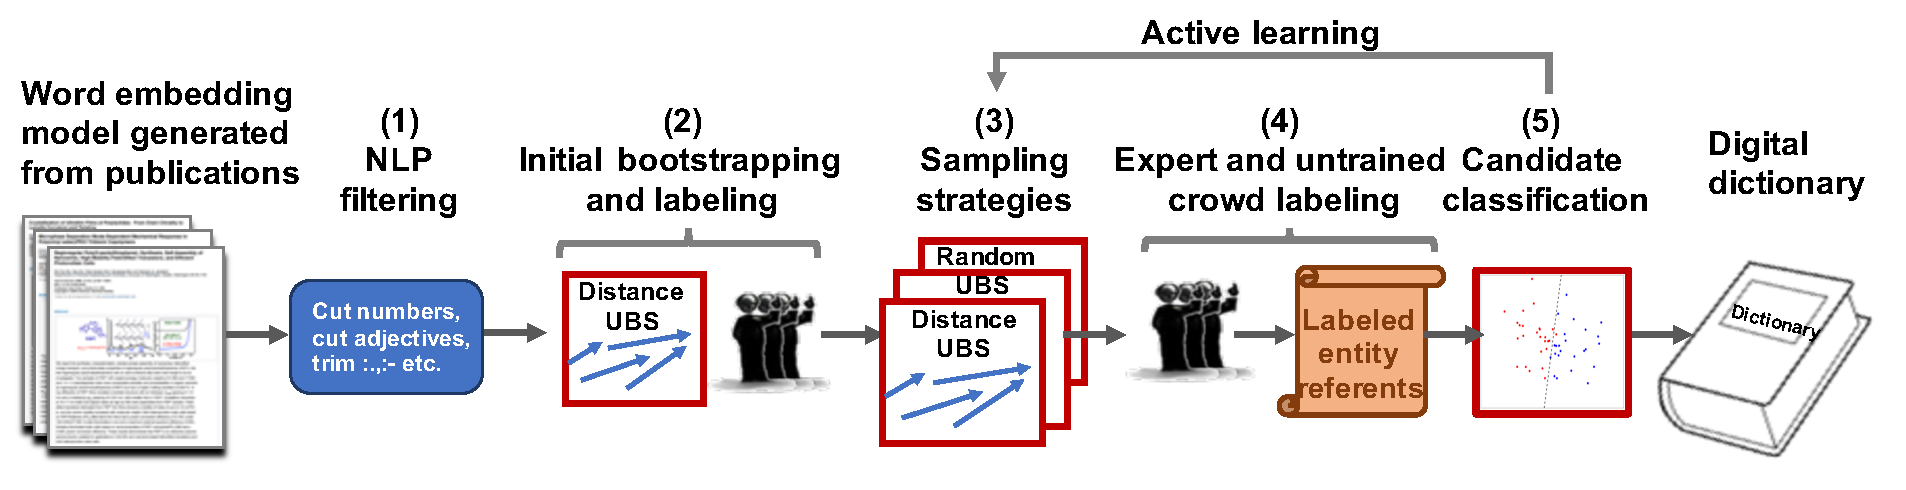
\includegraphics[width=\textwidth]{figures/architecture.pdf}}
\caption{\label{fig:architecture} PolyNER system showing the different phases of polyNER including the NLP-filtering step, the initial bootstrapping and labeling phase as well as the newly integrated active learning loop to classify scientific named entities. 
%\ian{(1) It is really important to be consistent in how your refer to things. Here, the figure says ``Bootstrapping and Initial Labeling" for (1), but the caption says ``initial sampling and labeling.'' Pick one and use it consistently. (2) You are inconsistent in capitalization. (3) The caption mostly repeats the labels in the figure, which seems redundant.
%It could be higher level.}
	%\logan{Should we differentiate between the "initial sampling" strategy done to bootstrap our training set and the "active learning sampling" strategy used to identify the next things to label? Mixing the two up is going to confuse people}\roselyne{OK will adapt the rest of the text and section titles too.}
}
\end{figure*}

\subsection{Computing Word Embeddings}\label{sec:wordembeddings}
A word embedding method maps each word
in a document to a vector in an n-dimensional real vector space that
represents the linguistic context in which the word appears. This mapping may
be based, for example, on co-occurrence frequencies of words. 
We can then determine the similarity between two words by computing the distance between
their corresponding vectors in the feature space.

We use Word2Vec, a recent, light-weight and easy-to-use implementation of context-based vector representations~\cite{mikolov2013efficient,mikolov2013distributed}.
Specifically, we use the Gensim continuous bag-of-words
(CBOW) implementation of the Word2Vec
algorithm~\cite{rehurek2010software} to generate vectors.
Based on prior parameter tuning we set the 
%We describe in Section~\ref{sec:wes} how we select appropriate values for the
Word2Vec \texttt{size} parameter to 100 and the \texttt{window_size} to 2; 
where \texttt{size}  is the size of the vector, and \texttt{window_size}
is an adjustable window of surrounding context word used to compute each embedding.

\subsection{NLP-Filtering}\label{sec:filter}
%\subsubsection{Word Embedding Model}
%\logan{Why is this titled "Word Embedding Model" and you start by describing a classifier?}
%We hypothesize that we can implement a classifier, which can detect word vectors for polymers based on their context. 
%\logan{This is the only section that you start with a "hypothesis"}\roselyne{ok removing this and moving section}
%\logan{Where is this section in F\ref{fig:architecture}?}
%We generate an unsupervised word embedding model using out entire corpus and train classifiers on vector representations using labels generated via the active learning(step 3 of Figure~\ref{fig:current}).
%Finally, in step 4, we test our classifiers against all the NLP-filtered words from the test corpus, as shown on Figure~\ref{fig:current}.

The NLP filtering preprocessing step removes strings that are unlikely to be polymer referents. 
First, we remove
unwanted characters (e.g. `:', `.', `,', `:', `-') from the beginning and the end of each
candidate, and eliminate numbers (including numbers followed by common units).
This step allows us to recognize, for example, ``polyethylene;'' (with the extraneous `;') 
as a duplicate of ``polyethylene''. 
Hypothesizing that names of scientific entities will not, in general, be English
vocabulary words, we also remove words found in the SpaCy dictionaries
of commonly used English words~\cite{choi2015depends}. We manually remove common polymer
names, such as polystyrene and polyethylene, from the dictionaries.
We also use
SpaCy's part-of-speech tagging functionality to remove non-nouns.  
Finally, we remove plurals (e.g.,
polyamides, polynorbornenes), as they can represent polymer family names.
Note that these steps are generalizable and applicable to multiple science fields.
We refer to the set of words that results when these filtering operations are applied to our corpus 
as the \emph{NLP-filtered candidates}.
This set is the output of step 1 in Figure~\ref{fig:architecture}.

\subsection{Initial Bootstrapping and Labeling}\label{sec:initial}
NLP filtering reduces the number of entities to be considered, and increases the target vs.\ non-target entity ratio.
However, there still remain a large pool of potential candidates from which entities are to be selected,
of which, in our experience, roughly 5\% are polymer names.
In order to avoid presenting experts with mostly negative examples, hindering meaningful classification,
we boost the number of polymer entities in the first batch of candidates to be annotated by
selecting strings with low word vector distance (see Section~\ref{sec:wordembeddings}) from
a set of \emph{seed entities}:
words that are observed to occur frequently  
in a subset of publications, or that are suggested by experts.
We discuss this distance metric in more detail below.
Based on preliminary experiments, we set the size of each batch of strings to be labeled to 200, 
or about an hour of expert time.
We then train the initial classifier on this bootstrap set, using 80\% of the data for training and 20\% for testing.
We subsequently used three different sampling strategies for following classifications.


%\subsection{Bootstrapping}\label{sec:bootstrap}
%%Having explored the parameters for distance candidate generation, we generate a pool of \num{10000} candidates most similar to the three most frequent polymers and their acronyms from a test corpus of \num{1690}, excluding any token found in our test documents. 
%%\logan{Is the 10k entries mentioned in the previous section this set? If so, we need to revise the order of these sections?}
%The UBS and Distance UBS sampling methods use a classifier to 
%determine which NLP-filtered entities should be chosen next for expert labeling.
%This classifier must be trained, and thus we need an initial set of entities to bootstrap this process.
%We could choose NLP-filtered entities at random for initial labeling, 
%but that choice is unlikely to perform well due to the low proportion of polymers (just 5\%) in the NLP-filtered corpus.
%Instead, therefore, we create an initial bootstrap set comprising the 200 NLP-filtered entities 
%that are closest, in word distance vectors, to a set of seed entities.
%%\ian{I assert that there is no need to mention the \num{10000} number here: you just take the 200 with the lowest score, as the 10000 is just the ones with the lowest distance scores, yes?}\roselyne{yes, or highest similarity, I wonder if I should change my preference for distance, because distance implies, minimal distance but Word2Vec and FastText give similarity values, discuss.}
%(Recall that we use a batch size of 200 based on an estimate of 60 minutes of expert time required for labeling.)
%We then train the initial classifier on this bootstrap set, using 80\% of the data for training and 20\% for testing.

%\ian{I will come back and look at this later, but I want to make a note for now.
%Section~\ref{sec:initial} and Section~\ref{sec:bootstrap} are basically duplicates: they both describe
%the bootstrap process. We need to work out whether this is better stated before or after the sampling
%strategy material.}\roselyne{You are right, changing the figure to say initial bootstrapping and labeling, it is the same step}

\subsection{Sampling Strategies}\label{sec:sampling}
%While the previous steps reduces the numbers of candidates and the imbalance of the dataset (target vs. non-target entity ration), there still remains a relatively large pool of potential candidates to select entities from.
%In order to achieve higher classification accuracy\textemdash
%by decreasing the number of potential false positives (candidates incorrectly identified as targets by our classifier)
%\textemdash we want to carefully select examples to be labeled by experts.
%\logan{Why is labeling "false positives" bad?}\roselyne{It just takes more time from the expert, also we can't give the expert only negative examples.}
We implement three sampling strategies, which we refer to as \textit{Random}, \textit{Uncertainty-Based Sampling (UBS)} and \textit{Distance Uncertainty-Based Sampling (Distance UBS)}.
We apply each of these strategies to our NLP-filtered candidates to determine which candidates to present to experts for labeling.
%Based on preliminary experiments, we set the size of batches of strings to be labeled to 200 or about an hour of expert time.
%\logan{As my comment in F\ref{fig:architecture}, we have two different kinds of sampling strategies and I think we should describe them separately. What do you think?}\roselyne{I'm separating the initial sampling and adding it to the figure}

\subsubsection{Random}
Here, we randomly select 200 of the NLP-filtered candidates.
%IAN removed next two lines as we just said that above.
%Note that the imbalance between polymers and other NLP-filtered \textit{tokens} 
%(words or space-separated strings) is still significant (around 5\% in our experience).
%We exclude tokens included in our test set.\ian{I have no idea what the preceding text is saying. What does it mean to have an imbalance with things that do not exist?
%Could this paragraph simply be, ``As a baseline, we will present results for a random selection strategy,
%in which 200 candidates are selected at random from the NLP-filtered candidates.''}\roselyne{It's missing dictionary, that do not exist in the dictionary}
%\ian{Separate issue: as far as I know, you have not introduced the concept of a test set, so the reference to test set is confusing.}

\subsubsection{Uncertainty-Based Sampling (UBS)}
Our second strategy applies maximum entropy sampling to the NLP-filtered candidates. % from the full corpus of documents used in the random strategy.
%\logan{Same pool}
As previously mentioned, maximum entropy selection is an uncertainty sampling method that
identifies data points for which a classifier predicts outcomes that lie near the decision boundary 
between classes. 
Thus, when predicting whether or not a word vector represents a polymer, 
maximum entropy arises when the classifier assigns equal probability to the polymer and not-polymer cases.
As we have two classes, this equal probability is 0.5.
%For example, in our case, when predicting whether or not a word vector represents a polymer, 
%the classifier assigns equal probability to either case.
%\ian{Can we say, ``As we have two classes" rather than ``in the binary case"?}
%In the binary case, probabilities range from 0 to 0.5. 
%\ian{Why can't you have a probability of 1, for say ``polystyrene''?}\roselyne{You're right, you can have that, and the text is confusing, if you you have a probability of 1, then |1-0.5| gives you 0.5 and this will not be considered as a confusing example, the examples with probability p with |0.5-p| close to 0 are the ones considered confusing} 
We use the classifier to obtain a probability $p$ for each NLP-filtered candidate. 
We select the 200 entries for which $p$ is closest to 0.5 as our sample.

\subsubsection{Uncertainty-Based Sampling with Distance Ranking (Distance UBS)}
Our third strategy is identical to UBS, except that it works with just a subset of the NLP-filtered candidates,
namely the \num{10000} that are closest to a set of seed entities. 
The intuition here is that a candidate is more likely to be a target referent 
(a name, acronym, synonym, etc.) if it used in a similar context.
For example, the polymer name ``polystyrene'' in a sentence ``The
melting point of polystyrene is ...'' suggests that X may also be a polymer in the
sentence ``The melting point of X is ...''.

We use the word embeddings introduced in Section~\ref{sec:wordembeddings} to capture this notion of context,
and vector distance between word vectors as a measure of similarity.
Whether or not this approach works in practice will depend on whether 
polymer names are in fact used in consistent contexts as captured by our 
word embedding  vectors. 

We can then determine, for each NLP-filtered word, the extent to which it occurs
in a similar context to the seed entities, by computing the similarities
between the word's vector and those for our seed entities. 
As we explain in Section~\ref{sec:wes}, we experiment with one and more seed entities; 
when dealing with multiple seed entities,
we use the lowest distance score for ranking candidates.
%Here too, we exclude terms that exist in our test set of documents.



%\subsubsection{Initial Classifier}
\subsection{Bootstrapping}\label{sec:bootstrap}
%Having explored the parameters for distance candidate generation, we generate a pool of \num{10000} candidates most similar to the three most frequent polymers and their acronyms from a test corpus of \num{1690}, excluding any token found in our test documents. 
%\logan{Is the 10k entries mentioned in the previous section this set? If so, we need to revise the order of these sections?}
The UBS and Distance UBS sampling methods use a classifier to 
determine which NLP-filtered entities should be chosen next for expert labeling.
This classifier must be trained, and thus we need an initial set of entities to bootstrap this process.
We could choose NLP-filtered entities at random for initial labeling, 
but that choice is unlikely to perform well due to the low proportion of polymers (just 5\%) in the NLP-filtered corpus.
Instead, therefore, we create an initial bootstrap set comprising the 200 NLP-filtered entities 
that are closest, in word distance vectors, to a set of seed entities.
%\ian{I assert that there is no need to mention the \num{10000} number here: you just take the 200 with the lowest score, as the 10000 is just the ones with the lowest distance scores, yes?}\roselyne{yes, or highest similarity, I wonder if I should change my preference for distance, because distance implies, minimal distance but Word2Vec and FastText give similarity values, discuss.}
(Recall that we use a batch size of 200 based on an estimate of 60 minutes of expert time required for labeling.)
We then train the initial classifier on this bootstrap set, using 80\% of the data for training and 20\% for testing.
% in the previously discussed list of \num{10000} candidates.
%\logan{Maybe we can be specific here about how much time it took. "We found that a batch of 200 required ..."}\roselyne{this is an average based on your estimate, but I don't have an exact number from the first test}
%As shown in Figure~\ref{fig:current}, in the first step, we train and test on candidates generated from a word embedding model generated using only the training documents. 
%We train the classifier on 80\% of the data and test on 20\%.

\subsection{Active Learning Loop}\label{active_learning_loop}
We now discuss our active learning process. 
As discussed in Section~\ref{sec:active}, the basic idea here is that we repeatedly select a set of 200
candidate entities (a ``sample'') for expert labeling, 
based on what we have learned from previously labeled entities.
We run this process independently with the Random, UBS, and Distance UBS sampling strategies,
in order to compare their performance.
%We describe these steps in more details in the following sections.

\subsubsection{Use and Evaluation of Classifiers}
Not specified in Section~\ref{sec:sampling} is the nature of the classifier that the UBS and Distance UBS strategies
use to estimate the probability of each entity in the NLP-filtered corpus (or, for Distance UBS,
the \num{10000}-entity subset of the NLP-filtered corpus) being a polymer.
(The Random strategy does not use a classifier for sampling, as it selects candidates at random.)
As we have no prior knowledge of the distribution of target entities in the vector space, 
we consider seven distinct classifiers in each round of the active learning process:
the scikit-Learn~\cite{scikit-learn} implementations of Decision Tree,
%(DT), 
Gradient Boosting,
% (GB), 
K-Nearest Neighbor (KNN), 
Logistic Regression, 
%(LR), 
Linear Support Vector Machine,
% (SVM), 
Naive Bayes, 
%(NB), 
and Random Forest. % (RF).
In each case, we use the word embedding for each string as input features.
In each round $i$, we train these seven classifiers on the sample data gathered in rounds $j$, $j$<$i$,
and then use the classifier with the highest recall to determine the $p$ scores that UBS and Distance UBS use when
assembling their 200-entity sample in that step.
(We use recall, or retrieving a maximum of targets, as a measure of performance, because we want to favor
extracting a higher number of targets, potentially requiring additional curation, over obtaining fewer correct targets.)

%\ian{text from Kyle: Probably I will confuse things here further. At each phase of the AL cycle (200 labels) we train many classifiers (KNN, RF, other ones that I forget). We then take the best performing one (by recall I gather above) and use that to select the candidates for the next round. That process continues in each round. So in some rounds we might have KNN being used, in others it might be RF. I understand that it somewhat converges on KNN in the later rounds.}
%As we have no prior knowledge of the distribution of target entities in the vector space, 
%we use multiple classifiers at each round of the active learning process. 
%We use the best performing classifier on the labeled candidates for subsequent maximum entropy-based uncertainty sampling. 
%\logan{You have neither defined nor motivated MEU, I think}\roselyne{See if you would add something to the previous strategies (UBS). That's where I've tried to define it, tell me if it's not clear}.
The 200 entities in the new sample are passed to experts for annotation,
and the annotated data are added to the set of training data used in the next learning round.


\subsubsection{Expert (and Non-expert) Labeling}
%As explained in Section~\ref{sect:background}, recognizing polymers can require more or less domain expertise.
We engage two domain experts to annotate the candidates generated by the 
\textit{UBS} and \textit{Distance UBS} sampling strategies. 
Each expert annotates one strategy;
we also perform crosschecking for 10\% of the first batch of labels, to get a measure of agreement between experts,
with results reported in Section~\ref{sec:labeling}. 
%We confirm agreement between labels for all but 1 of the set of 20 candidates or an agreement of 95\%.
%\logan{The inter-relater score is a result, not part of the architecture}\roselyne{ok, don't remove, come back to this to make sure I add it later}
Experts use a web interface (see Figure~\ref{fig:polyner}) to approve or reject candidates,
a task that is far more efficient than reading and annotating words in text.
The interface
provides example sentences as context for ambiguous candidates
and allows the expert to access the publication(s) in which a particular candidate
appears. % when desired.

We aim to reduce the amount of costly expert time used to obtain labels.
%Expert time is costly and we aim to reduce the cost of obtaining labels.
Therefore, for our baseline of randomly sampled NLP-filtered nouns, we experiment with a two-phase review process.
Tokenization is one of the largest sources of error for scientific entities such as polymers, 
which contain characters such as `:', `(',
'\textendash', `,' etc. 
Tokenization can also generate incoherent tokens from text, equations, captions, etc.
Such obvious non-candidates can be fairly easily detected by non-experts.
For example, an untrained human annotator may be able to recognize that `$d\Sigma/d\Omega)(Q$' is not a polymer name, and thus save time for the experts.
Hence, we assigned two graduate student labelers to curate the candidates generated by the random sampling strategy, which are less likely to contain target entities.
We asked these untrained labelers to reject obvious non-candidates via the previously mentioned web interface. 
Our experts then reviewed the remaining
candidates, indicating for each whether it is in fact a polymer referent. % and submits a final review.

%While we first used this two-phase review process for the random strategy, 
%we envision generalizing and leveraging humans with different expertise through multi-phase reviews for all strategies to further save costs.


\begin{figure}
\centering
\frame{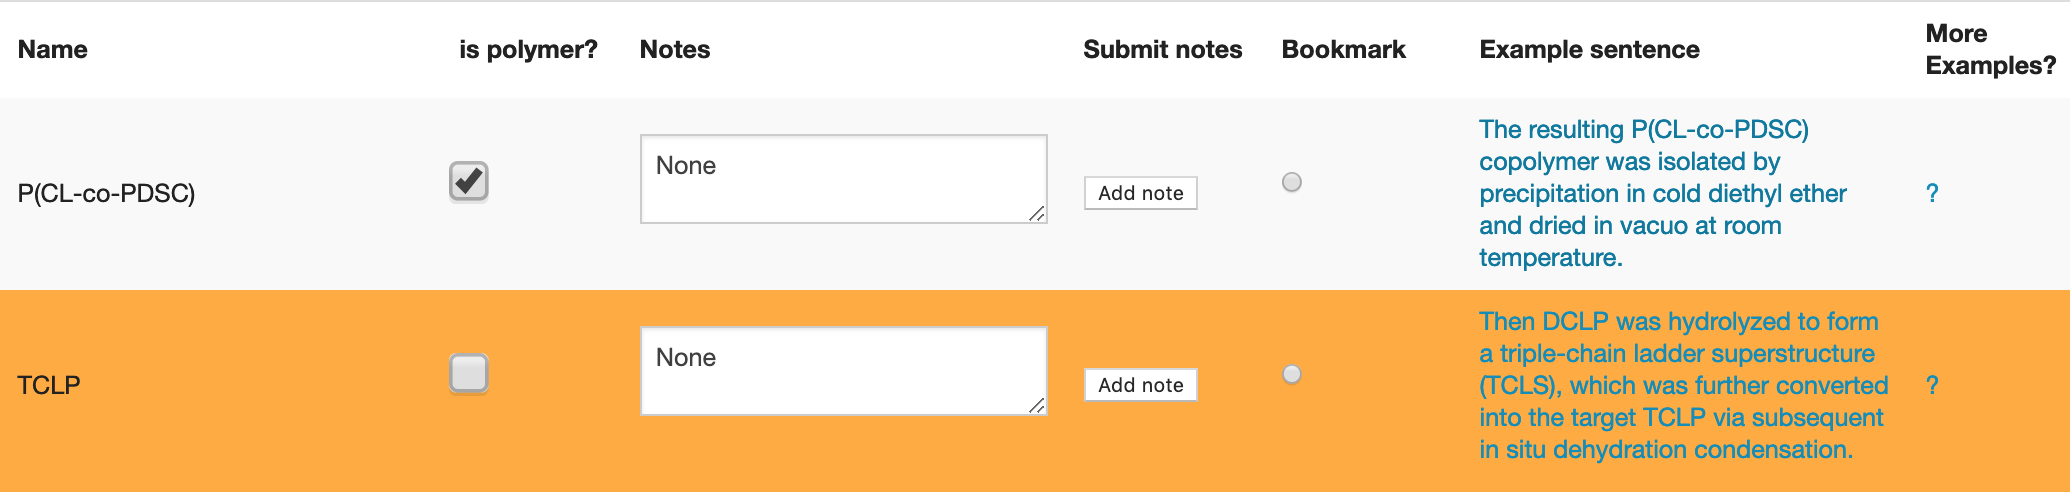
\includegraphics[trim=0in 0.1in 0.1in 0.in,clip,width=3.5in]{figures/expert_labeling.png}}
\caption{\label{fig:polyner} Web interface for expert review of candidates.
The expert indicates whether the name (column 1) is a polymer (tickbox in column 2), 
providing notes if desired (column 3). 
Clicking on ``?'' delivers up to 25 more example sentences.
}
\end{figure}

%\subsubsection{Classification or Candidate Discrimination}
%We use multiple classifiers that we concurrently trained and test on the same data in steps 1, 2, and 3 of Figure~\ref{fig:current}.
%\ian{I think that this subsubsection can be removed, as the rest of its contents are now above. 
%I am just not sure about the remaining sentence. I don't understand Figure 2, so I am not sure if it adds information.}\roselyne{Agreed and it is referring to an old version of the figure. I also fits in the active learning loop, so no need to have a new one.}
%The classifiers include the scikit-Learn~\cite{scikit-learn} implementations of Decision Tree (DT), Gradient Boosting (GB), K-Nearest Neighbor (KNN), Logistic Regression (LR), Linear Support Vector Machine (SVM), Naive Bayes (NB), and Random Forest (RF). 
%\logan{Something to consider for future: I've been nervous a long time about how we use so many models. How good is your grid search CV for these models? Many (KNN, SVM) are super sensitive to hyperparameters, and I'm worried we are testing 7 models badly and that we'd have better results with tuning 1 really well}
%\roselyne{Yes, this is definitely a lesson taken. I was just telling Kyle, I know exactly how I would change this experiment and others based on my experience now. Perhaps I need to say that in the discussion!}\roselyne{Added note to include in discussion}
%Our goal here is to explore the word embedding space and determine which classifier(s) works best for detecting our scientific named entities.
%As previously mentioned, we select the best-performing classifier on labeled candidates for subsequent uncertainty sampling.

%\logan{Can you express this quantitatively?}\roselyne{I have favored recall, maybe I should just say that? better?}
%\logan{Do you mean "use the word embedding for each word as input"? All word vectors should have the same dimensions}\roselyne{yes, they do, I want to indicate exactly that the valye of the dimensions word vector itself is used as features, I wasn't sure if the embedding for each word as input was clear enough.}




